\documentclass[pagesize=pdftex,paper=a4,fontsize=12pt]{scrartcl}


\usepackage[english]{babel} % Neue Rechtschreibung, Inhaltsverzeichnis, ...
\usepackage[utf8]{inputenc} % Umlaute
\usepackage[T1]{fontenc} % vorgefertigte zusammengesetzte Zeichen
\usepackage{lmodern}
\usepackage{amsmath} % Mathematikumgebung
\usepackage{amssymb} % Mathsymbole
\usepackage{array} % Tabellen
\usepackage{graphicx} % Bilder einfügen
\usepackage{hyperref}
\usepackage{pgfplots}
\usepackage{siunitx}
\usepackage{svg}
\usepackage{float}

\usepackage{tikz} % Grafiken
\usetikzlibrary{arrows, decorations.pathmorphing, calc}

\title{Rainbows}
\author{Johannes Wilde}

\newcommand{\abs}[1]{\ensuremath{\left|{#1}\right|}}
\newcommand{\R}{\mathbb{R}}

\setlength{\oddsidemargin}{-1cm}
\setlength{\textwidth}{18cm}
\setlength{\topmargin}{-1.5cm}
\setlength{\textheight}{24cm}

\begin{document}

\maketitle

\section{Geometrical Assumptions}

A raindrop is assumed to be perfectly circular, its radius normalized to $1$ and the inside and outisde described via refractive inidices $n_1$ and $n_0$.

\begin{figure}[H]
	\centering
	\includesvg[width=15cm]{PrincipleSketch.svg}
	\caption{Principle scetch of the geometrical properties of a circular raindrop.}
	\label{fig:PrincipleScetch}
\end{figure}

From this simple sketch the following relations can be deduced:

\[ h = \sin(\alpha), \]

where Snell's law states:

\[ n_0 \sin(\alpha) = n_1 \sin(\beta), \]

\[ \varepsilon = \alpha - \beta, \]

\[ \zeta = [\SI{180}{\degree} - 2 \beta] / 2 = \SI{90}{\degree} - \beta, \]

\[ \delta = \SI{180}{\degree} - [[\SI{180}{\degree} - 2 \beta] + \varepsilon] = 2 \beta - [\alpha - \beta] = 3 \beta - \alpha, \]

\[ \gamma = \SI{180}{\degree} - 2 [\zeta + \varepsilon] = \SI{180}{\degree} - 2 [\SI{90}{\degree} - \beta + \alpha - \beta] = 2 [2 \beta - \alpha], \]

\begin{align}
	\gamma (\alpha) & = 2 \left[2 \arcsin\left(\frac{n_0}{n_1} \sin(\alpha)\right) - \alpha\right], \nonumber \\[.5em]
	\gamma (h) & = 2 \left[2 \arcsin\left(\frac{n_0}{n_1} h\right) - \arcsin(h)\right].
\end{align}

These relations are shown in figure \ref{fig:GammaOverH}. Please note that the plot for $\frac{n_0}{n_1} = 1$ shall only be understood as a border-case [$\lim_{\frac{n_0}{n_1} \to 1} \gamma (h)$] - physically there would be no such effect for homogenous refractive indices.

\begin{figure}[H]
	\centering
	\begin{tikzpicture}
	\begin{axis}[
		scale=1.5,
		domain=-1:1,
		samples=500,
		xlabel={$h\,[\text{normalized}]$},
		ylabel={$\gamma\,[\si{\degree}]$},
		legend pos=north west,
		legend columns=2,
		cycle list name=color list
	]
		\foreach \refractiveIndexRelation in {1.00, 1.05, 1.10, 1.15, 1.20, 1.30, 1.40, 1.60, 1.80, 2.00, 2.40, 2.80}
		{
			\addplot +[mark=none] (x, {2 * (2 * asin(x/\refractiveIndexRelation) - asin(x))});
			\expandafter\addlegendentry\expandafter{\expandafter$\refractiveIndexRelation\expandafter$};
		}
	\end{axis}
	\end{tikzpicture}
	\caption{Excidence angle $\gamma$ over incidence height $h$.}
	\label{fig:GammaOverH}
\end{figure}

\pagebreak

\section{Extrema}

The derivate is [using $\frac{d}{dx} \arcsin(x) = \frac{1}{\sqrt{1-x^2}}$]:

\[ \frac{d}{dh} \gamma (h) = 2 \left[2 \frac{n_0}{n_1} \frac{1}{\sqrt{1-[\frac{n_0}{n_1} h]^2}} - \frac{1}{\sqrt{1-h^2}}\right]. \]

Thus the local extrema are:

\newcommand{\hExtremum}{\ensuremath{h_{\text{extr.}}}}
\newcommand{\gammaExtremum}{\ensuremath{\gamma_{\text{extr.}}}}
\begin{align}
	0 & \stackrel{!}{=} \frac{d}{dh} \gamma (\hExtremum)\\
 & = 2 \left[2 \frac{n_0}{n_1} \frac{1}{\sqrt{1-[\frac{n_0}{n_1} \hExtremum]^2}} - \frac{1}{\sqrt{1-\hExtremum^2}}\right], \nonumber \\[.5em]
	\frac{1}{\sqrt{1-\hExtremum^2}} &= 2 \frac{n_0}{n_1} \frac{1}{\sqrt{1-[\frac{n_0}{n_1} \hExtremum]^2}}, \nonumber \\[.5em]
	1-\left[\frac{n_0}{n_1} \hExtremum\right]^2 &= \left[2 \frac{n_0}{n_1}\right]^2 \left[1-\hExtremum^2\right], \nonumber \\[.5em]
	\left[\frac{n_1}{2 n_0}\right]^2 -\left[\frac{1}{2} \hExtremum\right]^2 &=  1-\hExtremum^2, \nonumber \\[.5em]
	\frac{3}{4} \hExtremum^2 &=  1 - \left[\frac{n_1}{2 n_0}\right]^2, \nonumber \\[.5em]
	\hExtremum^{\pm} &= \pm \sqrt{\frac{1}{3} \left[4 - \left[\frac{n_1}{n_0}\right]^2\right]}.
\end{align}

From this one finds:

\begin{equation}
	 1 < \frac{n_1}{n_0} \leq 2.
\end{equation}

And the angle values at these local extreme are:

\begin{equation}
	\gammaExtremum^{\pm} = \gamma (\hExtremum^{\pm}) = \pm 2 \left[2 \arcsin\left(\frac{n_0}{n_1} \sqrt{\frac{1}{3} \left[4 - \left[\frac{n_1}{n_0}\right]^2\right]}\right) - \arcsin\left(\sqrt{\frac{1}{3} \left[4 - \left[\frac{n_1}{n_0}\right]^2\right]}\right)\right].
\end{equation}


\begin{figure}[H]
	\centering
	\begin{tikzpicture}
	\begin{axis}[
	scale=1.5,
	domain=1:2,
	samples=500,
	xlabel={$\frac{n_1}{n_0}$},
	ylabel={$\gammaExtremum^{+}\,[\si{\degree}]$},
	legend pos=north west,
	legend columns=1,
	cycle list name=color list
	]
		\addplot[mark=none] (x, { 2 * (2 * asin(sqrt((4-x^2)/3)/x) - asin(sqrt((4-x^2)/3))) });
		\node[label={0:{water @ \SI{550}{\nano\meter}}},circle,fill,inner sep=2pt] at (axis cs:1.334683329053798,41.83394805963984) {};
	\end{axis}
	\end{tikzpicture}
	\caption{Excidence angle $\gamma{+}$ over incidence height $h$.}
	\label{fig:GammaMaxOverRefractiveIndexRelation}
\end{figure}

For water at \SI{20}{\degreeCelsius} and light of \SI{550}{\nano\meter} [$n_0 = 1$, $n_1 = 1.3347$] this yields an angle of $\gammaExtremum^{+} = \SI{41.83}{\degree}$.


Because of what will be shown in the next section, this also corresponds to the angles of maximum power density excidence.


\section{Power Density Superelevation}



\begin{figure}[H]
	\centering
	\begin{tikzpicture}
	\begin{axis}[
	scale=1.5,
	domain=.75:.9,
	samples=500,
	xlabel={$h\,[\text{normalized}]$},
	ylabel={$\gamma\,[\si{\degree}]$},
	legend pos=north east,
	legend columns=1,
	cycle list name=color list
	]
	\addplot +[mark=none] (x, {2 * (2 * asin(x/1.3347) - asin(x))});
	\addlegendentry{$1.3347$};
	\addplot +[samples=11, mark=*] (x, {2 * (2 * asin(x/1.3347) - asin(x))});

	\draw (axis cs: 0.765, 39.57509140415948) -- (axis cs: 0.765,40.07022730844841) -- (axis cs: 0.75,40.07022730844841);
	\draw (axis cs: 0.78, 39.57509140415948) -- (axis cs: 0.78,40.52158477595456) -- (axis cs: 0.75,40.52158477595456);
	\draw (axis cs: 0.7725, 39.57509140415948) node {$\Delta h_{i}$};
	\draw (axis cs: 0.75, 40.29590604220148) node[anchor=east] {$\Delta \gamma_{i}$};
	\draw (axis cs: 0.855, 39.57509140415948) -- (axis cs: 0.855,41.82485632231572) -- (axis cs: 0.75,41.82485632231572);
	\draw (axis cs: 0.87, 39.57509140415948) -- (axis cs: 0.87,41.80216101831409) -- (axis cs: 0.75,41.80216101831409);
	\draw (axis cs: 0.8625, 39.57509140415948) node {$\Delta h_{j}$};
	\draw (axis cs: 0.75, 41.8135086703149) node[anchor=east] {$\Delta \gamma_{j}$};
	
	\end{axis}
	\end{tikzpicture}
	\caption{Excidence angle $\gamma$ over incidence height $h$.}
	\label{fig:GammaOverHExcerpt}
\end{figure}

As the incident power density $p_h$ is written in terms of $h$ [where the total power is $P = \int_\R p_h (x) dx$] it has to be transformed when changing the underlying coordinates. This is accomplished as followes:

\[ p_{\gamma} (x) = \sum_{y~|~x = \gamma(y)} p_h (y) ~ \abs{\frac{1}{\displaystyle \left.\frac{d\gamma (z)}{dz}\right|_{z=y}}} \]

which ensures that $P = \int_{\R} p_{\gamma} (x) dx$.

This can be seen in figure \ref{fig:GammaOverHExcerpt}, where the power incident e.g. in $\Delta h_{j}$ [$= \int_{h_j}^{h_{j+1}} p_h (x) dx$] exits in a much smaller angle region $\Delta \gamma_{j}$ compared to the power incident in $\Delta h_{i}$ --- which in return means that the power density $p_\gamma$ has to be much higher for $\gamma_j$ than for $\gamma_i$.

\begin{figure}[H]
	\centering
	\begin{tikzpicture}
	\begin{axis}[
	scale=1.5,
	domain=.75:.9,
	ymax=50,
	samples=500,
	xlabel={$h\,[\text{normalized}]$},
	ylabel={$\gamma\,[\si{\degree}]$},
	legend pos=north east,
	legend columns=1,
	cycle list name=color list
	]
	\addplot +[mark=none] (x, {1 / 2 / abs(2 / 1.3347 / sqrt(1 - (x/1.3347)^2) - 1 / sqrt(1 - x^2))});
	\addlegendentry{$1.3347$};
		
	\end{axis}
	\end{tikzpicture}
	\caption{Power density scaling $\abs{\frac{1}{\displaystyle \left.\frac{d\gamma (z)}{dz}\right|_{z=y}}}$ just because of the geometry.}
	\label{fig:invdGammadHOverHExcerpt}
\end{figure}

Because $\gamma (h)$ exhibits a local extremum the derivative becomes $0$ and thus the absolute value of its inverse $\infty$ at that point. Regarding numerical calculations this is a major inconvenience. It however justifies to only consider the geometrical relations for this investigation.

\vspace*{\fill}

This however requires, that no other physcial effects annihilate all power transmitted at that extremum. I checked Fresnel for water and found the following:
\begin{figure}[H]
	\centering
	\includegraphics[trim={0cm 4.12cm 0cm 1cm}, clip, width=12cm]{./Images/results_550.00.png}
	\caption{Angle and transmitted power in terms of Fresnel over $h$ [$\text{eta0} = -\gamma$].}
	\label{fig:waterFresnell}
\end{figure}


\end{document}